\documentclass[12pt]{article}
\usepackage{amsmath}
\usepackage{amssymb}
\usepackage[letterpaper,margin=0.85in,centering]{geometry}
\usepackage{fancyhdr}
%\usepackage{enumerate}
%\usepackage{lastpage}
\usepackage{multicol}
\usepackage{graphicx}
\usepackage{tikz}
\usetikzlibrary{calc, positioning, decorations.pathmorphing}

\reversemarginpar

\pagestyle{fancy}
\cfoot{}
\lhead{Math 1560}\chead{Tutorial Assignment \# 1 Solutions}\rhead{May 10th, 2017}
%\rfoot{Total: 10 points}
%\chead{{\bf Name:}}
\newcommand{\points}[1]{\marginpar{\hspace{24pt}[#1]}}
\newcommand{\skipline}{\vspace{12pt}}
%\renewcommand{\headrulewidth}{0in}
\headheight 30pt

\newcommand{\di}{\displaystyle}
\newcommand{\abs}[1]{\lvert #1\rvert}
\newcommand{\len}[1]{\lVert #1\rVert}
\renewcommand{\i}{\mathbf{i}}
\renewcommand{\j}{\mathbf{j}}
\renewcommand{\k}{\mathbf{k}}
\newcommand{\R}{\mathbb{R}}
\newcommand{\aaa}{\mathbf{a}}
\newcommand{\bbb}{\mathbf{b}}
\newcommand{\ccc}{\mathbf{c}}
\newcommand{\dotp}{\boldsymbol{\cdot}}
\newcommand{\bbm}{\begin{bmatrix}}
\newcommand{\ebm}{\end{bmatrix}}                   
                  

\begin{document}

%\author{Instructor: Sean Fitzpatrick}
\thispagestyle{fancy}
%\noindent{{\bf Name and student number:}}

 \begin{enumerate}
 \item  Solve the following inequalities:
\begin{enumerate}
 \item $x^2-2x\geq 15$

\bigskip

We have
\[
 x^2-2x\geq 15\Leftrightarrow x^2-2x-15\geq 0 \Leftrightarrow (x+3)(x-5)\geq 0.
\]
The sign diagram for this inequality is given by
\begin{center}
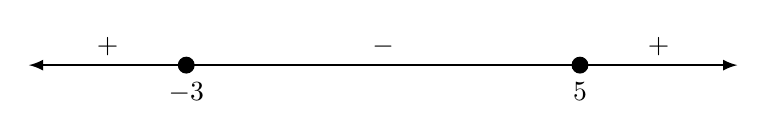
\begin{tikzpicture}[>=latex]
  \draw [thick, <->] (-5,0) -- (4,0);
  \draw [fill] (-3,0) circle [radius =.1];
  \draw [fill] (2,0) circle [radius =.1];
  \node at (-4,0) [above] {$+$};
  \node at (-0.5,0) [above] {$-$};
  \node at (3,0) [above] {$+$};
  \node at (-3,-0.1) [below] {$-3$};
  \node at (2,-0.1) [below] {$5$};
  \end{tikzpicture}
\end{center}

From the sign diagram we see that $(x+3)(x-5)\geq 0$ for $x\in (-\infty,-3]\cup[5,\infty)$.

 \item $1+\dfrac{3}{x+1}\leq\dfrac{4}{x}$

\bigskip

Rearranging, we have
\[
 1+\dfrac{3}{x+1}\leq\dfrac{4}{x} \Leftrightarrow \frac{x(x+1)+3x-4(x+1)}{x(x+1)}\leq 0 \Leftrightarrow \frac{x^2-4}{x(x+1)}\leq 0 \Leftrightarrow \frac{(x-2)(x+2)}{x(x+1)}\leq 0.
\]
To solve the inequality, we construct the sign diagram for the left-hand side. We find:
\begin{center}
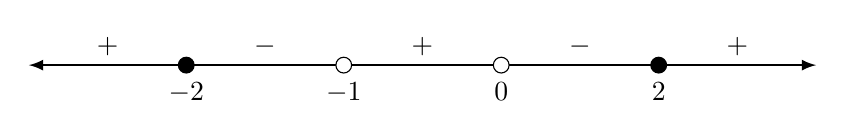
\begin{tikzpicture}[>=latex]
  \draw [thick, <->] (-5,0) -- (5,0);
  \draw [fill] (-3,0) circle [radius =.1];
  \draw [fill=white] (-1,0) circle [radius =.1];
  \draw [fill=white] (1,0) circle [radius =.1];
  \draw [fill] (3,0) circle [radius =.1];
  \node at (-4,0) [above] {$+$};
  \node at (-2,0) [above] {$-$};
  \node at (-0,0) [above] {$+$};
  \node at (2,0) [above] {$-$};
  \node at (4,0) [above] {$+$};
  \node at (-3,-0.1) [below] {$-2$};
  \node at (-1,-0.1) [below] {$-1$};
  \node at (1,-0.1) [below] {$0$};
  \node at (3,-0.1) [below] {$2$};
  \end{tikzpicture}
\end{center}
From the sign diagram, we see that the solution to the inequality is given by $x\in [-2,-1)\cup(0,2]$. \\
(Note that we do not include $0$ or $-1$ since the expression $\dfrac{(x-2)(x+2)}{x(x+1)}$ is not defined at these points. This is indicated on the sign diagram by using hollow dots.)
\end{enumerate}

\bigskip

\item Give a one-sentence explanation (in words) why the following are true:
\begin{enumerate}
 \item $\di \lim_{x\to a} b = b$ for any real numbers $a$ and $b$.

\medskip

Consider the constant \textit{function} $f(x)=b$. To say that $f(x)$ has limit $b$ as $x\to a$ is to say that we can make the value of $f(x)$ as close to $b$ as we want by taking $x$ sufficiently close to $a$. But the value of $f(x)$ is \textit{equal} to $b$ for \textit{all} $x$, so this condition is satisfied automatically.

 \item $\di \lim_{x\to a} x = a$ for any real number $x$.

\medskip

If we consider the function $g(x)=x$, we are saying that we can make the value of $g(x)$ as close to $a$ as we want by making $x$ sufficiently close to $a$. But since $g(x)=x$, making $g(x)$ close to $a$ is the same thing as making $x$ close to $a$.
\end{enumerate}

\newpage

\item Using properties of limits and the facts given in Problem \#2, show that for any \textit{polynomial} $p(x)$, and any real number $a$, we have $\di \lim_{x\to a}p(x)=p(a)$.

\bigskip

Let $p(x)=c_nx^n+c_{n-1}x^{n-1}+\cdots + c_1x+c_0$ be our polynomial function. We wish to show that
\[
 \lim_{x\to a}p(x) = c_na^n+c_{n-1}a^{n-1}+\cdots + c_1a+c_0 = p(a).
\]
From Problem 2(a) we know $\di\lim_{x\to a}(c_0)=c_0$, and using the product rule for limits with 2(a) and 2(b), we have
\[
 \lim_{x\to a}(c_1x) = (\lim_{x\to a}(c_1))(\lim_{x\to a}(x)) = c_1a.
\]
Similarly, for $k=2, 3, \ldots, n$, the power rule gives us $\di\lim_{x\to a}(c_kx^k) = c_k\left(\lim_{x\to a}(x)\right)^k = c_ka^k$. 

Using this, together with the sum rule, we have
\begin{align*}
 \lim_{x\to a}p(x) & = \lim_{x\to a}(c_nx^n+c_{n-1}x^{n-1}+\cdots + c_1x+c_0)\\
 & = \lim_{x\to a}(c_nx^n) + \lim_{x\to a}(c_{n-1}x^{n-1}) + \cdots + \lim_{x\to a}(c_1x) + \lim_{x\to a}(c_0)\\
 & = c_na^n + c_{n-1}a^{n-1}+\cdots + c_1a+c_0 = p(a), 
\end{align*}
which is what we wanted to show.

\bigskip

\item Evaluate each of the following limits, or explain it does not exist.
\begin{enumerate}
 \item $\di \lim_{x\to 3}\frac{x^2-9}{x^2-5x+6} = \lim_{x\to 3}\frac{(x-3)(x+3)}{(x-3)(x-2)} = \lim_{x\to 3}\frac{x+3}{x-2} = \frac{3+3}{3-2} = 6.$

\vspace{0.5in}

 \item $\di \lim_{x\to 2}\frac{x^2+4}{x-2}$ does not exist. Notice that as $x\to 2$ the denominator is approaching $2-2=0$, while the numerator is approaching $2^2+4=8$. Thus, as $x$ approaches 2, the value of $\dfrac{x^2+4}{x-2}$ increases without bound.

\medskip

Also acceptable: $\di \lim_{x\to 2^-}\frac{x^2+4}{x-2} = -\infty$, while $\di \lim_{x\to 2^+}\frac{x^2+4}{x-2} = +\infty$. Since the left and right hand limits do not agree, the limit does not exist. (We didn't discuss this approach in class, however, so I wasn't really expecting it.)

\newpage

 \item $\di \lim_{x\to 0}\frac{\sin(3x)}{\tan(5x)}$

\medskip

We employ a bit of algebraic manipulation to make use of known limits from class. Recall that $\di\lim_{\theta\to 0}\frac{\sin\theta}{\theta} = 1$; this result holds in particular for $\theta = 3x$ and $\theta =5x$ if $x$ is approaching 0. We have
\begin{align*}
 \lim_{x\to 0}\frac{\sin(3x)}{\tan(5x)} & = \lim_{x\to 0}\frac{\sin(3x)}{\sin(5x)/\cos(5x)} = \lim_{x\to 0}\frac{\sin(3x)}{\sin(5x)}(\cos(5x))\\
 & = \lim_{x\to 0} \frac{3}{5}\left(\frac{\sin(3x)}{3x}\right)\left(\frac{5x}{\sin(5x)}\right)(\cos(5x))\\
 & = \frac{3}{5}(1)(1)(1) = \frac{3}{5}.
\end{align*}
Notice that the expression in the second line is equal to that at the end of the first: the additional terms all cancel out. Note also that we've made use of the fact that
\[
 \lim_{x\to 0}\frac{5x}{\sin(5x)} = \lim_{x\to 0}\frac{1}{\dfrac{\sin(5x)}{5x}} = \frac{1}{\di\lim_{x\to 0}\frac{\sin(5x)}{5x}} = \frac{1}{1}=1.
\]

\end{enumerate}


 \end{enumerate}
\end{document}